\documentclass[12pt]{article}
\usepackage{amsmath, amssymb, fullpage}
\usepackage{array}
\usepackage{graphicx,psfrag,epsf}
\usepackage{enumerate}
\usepackage{caption}
\usepackage{subcaption}


\begin{document}

\title{Bayesian Hierarchical Models for Common Components across Multiple System Configurations}

\begin{abstract}
    We use a Bayesian hierarchical model to assess the reliability of the Joint Light Tactical
    Vehicle (JLTV), which is a family of vehicles. The proposed model effectively combines information
    across three phases of testing and across common vehicle components. The analysis yields
    estimates of failure rates for specific failure modes and vehicles as well as an overall estimate of the
    failure rate for the family of vehicles. We are also able to obtain estimates of how well vehicle
    modifications between test phases improve failure rates. In addition to using all data to improve on
    current assessments of reliability and reliability growth, we illustrate how to leverage the information
    learned from the three phases to determine appropriate specifications for subsequent testing that will
    demonstrate if the reliability meets a given reliability threshold.
\end{abstract}


\section{Introduction}

\section{Data}


\section{Methodology}

\subsection{Modeling Reliability}
A standard reliability analysis employed by the Department of Defense (DoD) test
community considers each test phase independently and uses the exponential
distribution to model the miles between failure ~\cite{ref1}. The traditional
analysis is overly simplistic, relies on correct modeling assumptions
and ignores valuable information learned about the individual vehicles and their
failure modes.

In considering the following alternative approach we will begin by introducing a
hierarchical model structure that can use data across all test phases and
incorporate known similarities between vehicle failure modes.  Next, we will
look at a number different modeling and distributional assumptions.  We discuss
different model diagnostics to consider when choosing a final model.  Then we
illustrate how this decision can effect our assessments of system reliability.
This will lead us into the next section on how this modeling can be used for
assurance test planning.

\subsubsection{Exponential Model}
In Test Phase 1, we assume the vehicle miles at failure, $y$, follow an
exponential distribution with a failure rate parameter $\lambda_{ij}$.
Introducing notation,
\begin{equation}
f(y_{ijk}|\lambda_{ij})=\lambda_{ij} \exp(-\lambda_{ij}
y_{ijk}), \quad i = 1,2,..,v \quad j=1,2,..,s \quad k=1,2,..,n_{ij}
\end{equation}
where $y_{ijk}$ are the miles between failure for vehicle $i$ failure mode $j$,
$v$ is the number of vehicles, $s$ is the number of failure modes, and $n_{ij}$
are the number of failures of vehicle $i$ failure mode $j$. The number of
failure modes is assumed fixed and known \textit{a priori}.

The prior distribution on the exponential failure rate parameter,
$\lambda_{ij}$, depends on whether failure mode $j$ is considered to be common
across vehicles or related but not identical. For the related failure modes,
we place a gamma prior distribution on the collection of $\lambda_{ij}$; in
other words, we assume each vehicle has a distinct failure rate in failure mode
$j$ but they arise from a common gamma distribution.

If failure mode $j$ is considered common across vehicles, the collection of
failure rates is collapsed to a single parameter, $\lambda_{ij} = \lambda_j$. As
with the related failure modes, a gamma prior distribution is placed on the
single failure rate. The prior distributions are independent across failure
mode, and can potentially have different hyperparameters.

The Phase 1 analysis yields an estimate of the failure rate $\lambda_{ij}$ for
each of the vehicles for failure modes that are related. We are assuming the
vehicles are conditionally independent, therefore the failure rate estimate for
the family of vehicles for such failure modes can be found by
$\sum_{i}\lambda_{ij}$. For failure modes that are common across vehicles the
Phase 1 analysis yields a $\lambda_{j}$, which is the failure rate for the
family of vehicles. Under the exponential modeling assumption the overall
failure rate across all failure modes can be found by $\sum_{j}\lambda_{j}$.

\subsubsection{Fix Effectiveness}
After the first CAP, Test Phase 2 begins with the repaired vehicles. To capture
these revisions, the PM2 reliability growth model \cite{EH06} is often used.
This model explicitly captures testing phases, choices about which failure modes
to correct, and the potential of not completely eliminating a failure upon
repair. One of the downsides of PM2 is that many parameters of potential
interest, such as the Fix Effectiveness Factor (FEF), which measures how much
repairs improve failure rates, are typically fixed. A common value for FEF is
0.70. We follow the premise of this type of model, but allow a more flexible and
data-driven result that is less dependent on hard-coded assumptions.

One normal assumption used in reliability growth modeling is non-decreasing
failure rates; that is either the fixes were effective or had no effect, but did
not degrade the family of vehicles.  This should generally be the case, but
because we are dealing with complex systems we will sometimes see decreases in
failure rates after adjustments are made.  Therefore for the Phase 2 data we
write the rate parameters as a function of the rate parameters found in Phase 1.
In particular, we define $\lambda_{ij}^{P2}=(\rho_{j})\lambda_{ij}^{P1}$ where
$\rho_{j}$ represents the between phase change in failure mode $j$. Given this
definition of $\lambda_{ij}^{P2}$, we again model the miles to failure for a given
vehicle and failure mode using the exponential distribution. We assume the prior
distribution for the $\rho_{j}$ is a gamma distribution.  If $\rho_{j}$ is less
than one, this represents an improvement in reliability.  After Phase 2 we can
look again at failure rates across failure modes and vehicles and obtain an
overall estimate of the rate for the family of vehicles.  The analysis of Test
Phase 3 follows the same pattern as that shown in Phase 2. At the end of
Phase 3, we can look at failure rates across failure m odes and vehicles and
obtain an overall estimate of the rate for the family of vehicles.
Future tests will be planned based on the inferences of Phase 3.

\subsubsection{Weibull Model}
The exponential model is by far the most common parametric distribution used in
reliability modeling because of its desirable math mathematical properties and
simple interpretations.   Despite its common uses the assumption of a constant
failure rate over time is rarely justifiable.  It has been well documented
(Statistics, Testing, and Defense Acquisition: Background Papers chapter - 2
http://www.nap.edu/catalog/9655.html) the issues that can arise when this
assumption is violated.  We will now consider the same hierarchical model
structure while using the Weibull distribution.  Now we assume that the failure
times $y_{ijk}$ each follow a $Weibull(\lambda, \gamma)$ distribution with scale
parameter $\lambda$ and shape parameter $\gamma$, with probability density
function
\begin{equation}
f(y_{ijk}|\lambda_{ij},\gamma_{i})=\lambda_{ij}\gamma_{i} y_{ijk}^{\gamma_{i}-1}\exp(-\lambda_{ij}
y_{ijk}^{\gamma_{i}}), \quad i = 1,2,..,v \quad j=1,2,..,s \quad k=1,2,..,n_{ij}
\end{equation}
The Weibull distribution is a more flexible model with both a rate parameter
$\lambda_{ij}$ and a shape parameter $\gamma_{j}$.  The exponential is a special
case of the Weibull, when $\gamma = 1$.
\\
It should be noted that we are currently indexing both $\rho$ and $\gamma$, only
by $j$ and not $i$, in other words we are assuming a single shape and rate
change parameter for each failure mode across vehicles.  All of these parameters
could also be indexed by $i$ and modeled hierarchical or with some combination
of both.  This is something we will omit for this paper but hope to explore in
the future.  One special case we will discuss is when a single shape parameter
can be assumed across all failure modes.  When this is justifiable it can
greatly simplify test planning calculations, as we will show in the assurance
testing section.

\subsubsection{JLTV Model Selection}
So far we have discussed a number of different models and the assumptions that
accompany them.  We will now discuss the process of model selection.  The
decision of which model to use can have a drastic impact on reliability
assessment and future test planning.  We will use the JLTV dataset to
demonstrate the process.

The first model selection question we will explore is the parametric form,
exponential versus Weibull.  In statistical modeling we often face the
trade-off between fit and interpretability, and this situation is no different.
Because the Weibull is a more flexible model, it will always, in a sense, fit the
data better, but this comes at a price.  The exponential's convenient form
makes both computation and interpretation straightforward.  When the Weibull's
shape parameter is introduced this advantage is lost.  Thus, when the overall
fit is close to the same between the exponential and the Weibull we will
default to using the exponential.

The first check we used to decide between the exponential and Weibull models is
to fit the Weibull model and look at the posterior distributions of the
shape parameters and determine if one is a reasonable value.  Looking at the
plot below from the JLTV data, we see that for the 26 components it appears
that the value of one falls in the extreme tails of the distributions.  This is
our first clue that the exponential model will not be a good fit to this data.

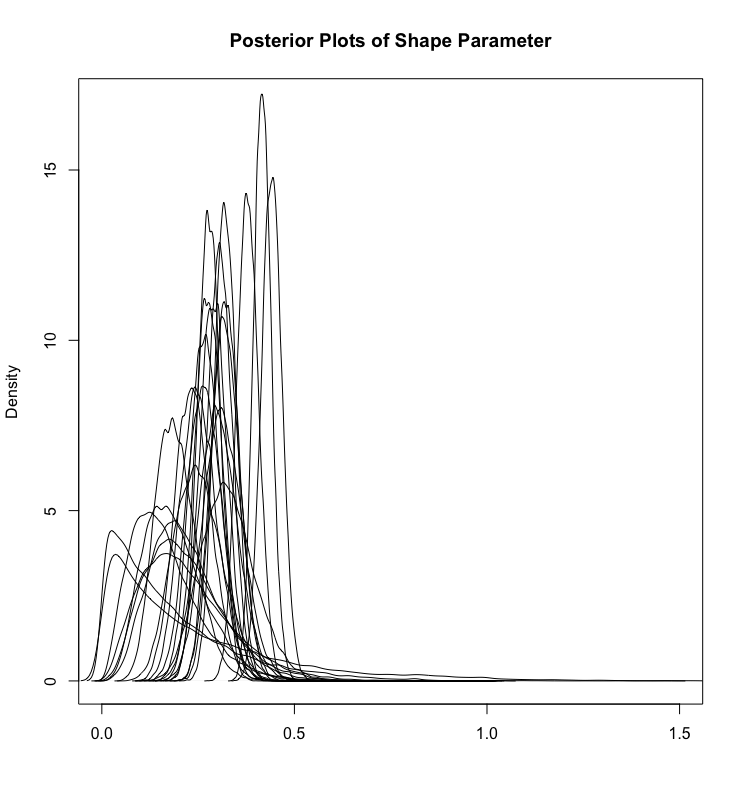
\includegraphics[width=6cm, height=5cm]{betaPostPlot}

This is not a surprising result, because the exponential model assumes constant
failure rate.  For most vehicle components we would expect the failure rate to
increase as the distance driven grows larger, and this corresponds with a shape
parameter between zero and one.  On the other hand, when the shape parameter is
larger than 1, the failure rate will decrease with time/distance.

Now a more formal diagnostic tool used for model selection is the Deviance
information criterion (DIC).  This is a popular method for comparing the
goodness of fit of multiple models.  The DIC method gives a slight penalty for
larger numbers of parameters.  The DIC value is a unitless measure with lower
values indicating a better fit to the data.  In the table below we show the DIC
results for the different distribution and structure combinations we considered
with the JLTV dataset.

\begin{tabular}{|l|l|r|}
\multicolumn{3}{c}{\textbf{Goodness of Fit}} \\
\cline{1-3}
Distribution    & Structure & DIC \\
\hline
Exponential   & Single Rate                       & 23258               \\
              & Hierarchical Rate                 & 23022               \\
Weibull       & Single Rate                       & 18750               \\
              & Hierarchical Rate                 & \textbf{18556}      \\
              & Hierarchical Rate (One shape)     & 18677               \\
\hline
\end{tabular}

The single rate structure represents the non-hierarchical model, using one rate
parameter all 8 vehicles for a given failure mode.  The hierarchical rate
structure uses the common gamma distribution for the failure modes that are
common across vehicles.  The final entry in the table is the model that uses one
shape parameter across all 26 failure modes.

While we have shown that the hierarchical Weibull model fits much better than
the exponential, these test still do not tell us that this model is a good fit
for the data.  The last method we will present is called posterior predictive
checking ***reference***.  Here we are given important features of the data.
In the JLTV case we were interested in the total failure counts for each phase
and the number of time the miles between failures was less than 140.  We then
used the final model to simulate 5,000 new datasets.  We then plot histograms
for each of the 8 vehicles for all 3 phases.  In Figure 1 are examples of the
histograms produced, with the line showing where the value of the true dataset
fell.  For this method we don’t expect all of the true values to fall in the
center of the distribution.  Values in the tales are to be expected in a random
processes like this one.  We will only be concerned if we find true values
falling in the extreme tails or if we see a common bias to the high or low side
of the distributions.

\begin{figure}
\centering
\begin{subfigure}{.5\textwidth}
  \centering
  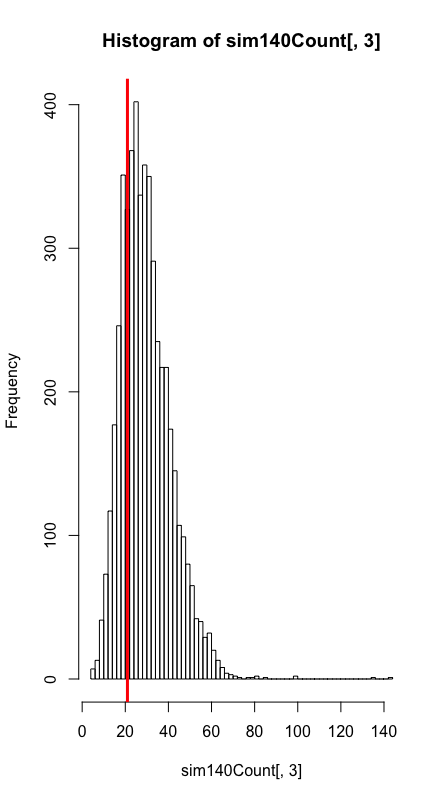
\includegraphics[width=.4\linewidth]{Rplot1}
  \caption{Plot 1}
  \label{fig:sub1}
\end{subfigure}%
\begin{subfigure}{.5\textwidth}
  \centering
  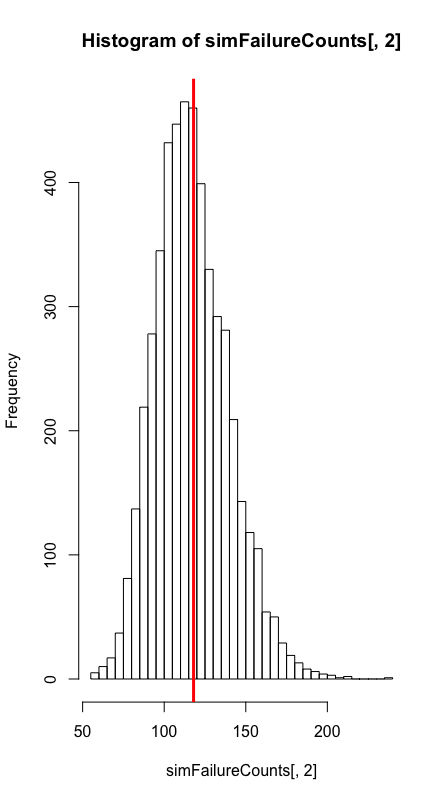
\includegraphics[width=.4\linewidth]{Rplot2}
  \caption{Plot 2}
  \label{fig:sub2}
\end{subfigure}
\caption{Posterior Predictive Plots}
\label{fig:test}
\end{figure}

\subsubsection{JLTV Reliability Results}

Results plots \\
Exponential vs. Weibull interpretation

\subsection{Assurance Test Planning}
In this section inferences learned from the first three phases of testing will
be used to develop a test plan for the next phase.  Here the objective is to
demonstrate that at a desired level of confidence, the system will meet or
exceed a specified requirement. The methods to be employed will be similar to
the assurance testing as discussed by Hamada et al. ~\cite{ref2}. Bayesian
assurance tests are used to insure that the reliability of an item meets or
exceeds a specified requirement with a desired probability. Although
practitioners often use ``assure'' and ``demonstrate'' synonymously, Meeker and
Escobar ~\cite{ME04} distinguish between reliability demonstration and
reliability assurance testing. A \emph{reliability demonstration test} is
essentially a classical hypothesis test, which uses only the data from the test
to assess whether the reliability-related quantity of interest meets or exceeds
the requirement. A \emph{reliability assurance test}, however, uses
supplementary data and information in order to testing as efficient as possible.

In both classical and Bayesian test planning scenario we are interested in
controlling error rates while minimizing the resources required for testing.  In
the DoD acquisition process the error rates will be referenced in terms of risk.
\emph{Consumer risk} which considers the event of purchasing a product that does
not meet reliability requirements.  \emph{Producer risk} which considers the
event of a product with acceptable reliability failing a given test and not
being considered for purchase.  Introducing the notation for this section, In
the JLTV case study we will be determining how many miles on test $T$, are
required and how many system failures to allow $c$, before the product is
considered unacceptable.  We will define $W(t)$ as a random variable that
represents the total number of system failures after $t$ miles.  Suppose that
$\pi$ denotes some quantity of interest that is related to system reliability at
a given time. It is common to base both classical and Bayesian test plans on two
specified levels of $\pi$: $\pi_0$, an \emph{acceptable reliability level}
(ARL), and $\pi_1$, a \emph{rejectable reliability level} (RRL), where $\pi_1
\leq  \pi_0$. Although the precise definition of ARL and RRL differ between the
classical and Bayesian test criteria, we use them in an equivalent way.

\subsubsection{Classical Approach}
It is quite common to use two criteria in determining classical test plans. The
\emph{producer's risk} is the probability of failing the test when $\pi =
\pi_0$, whereas the \emph{consumer's risk} is the probability of passing the
test when $\pi = \pi_1$.  Suppose that we specify a maximum value, $\alpha$, of
the producer's risk and a maximum value, $\beta$, of the consumer's risk. For
test planning, these criteria become
$$
\begin{aligned}
	\text{Producer's Risk} &= P \text{(Test Is Failed } \vert \pi_0 \text{)} \\
    &= P \text{(} W(t) > c \vert \pi_0 \text{)} \leq \alpha
\end{aligned}
$$
and
$$
\begin{aligned}
	\text{Consumer's Risk} &= P \text{(Test Is Passed } \vert \pi_1 \text{)} \\
    &= P \text{(} W(t) \leq c \vert \pi_1 \text{)} \leq \beta
\end{aligned}
$$
To choose a test plan for specified values of $(\alpha, \pi_0, \beta, \pi_1)$,
we assume a distributional form that defines the relationship between the number
of system failyres $W(t)$ and the reliability $\pi$.  Then we can simply find
the combinations of these probabilities by simultaneously solving these two
equations.  In the case where the component failure times are assumed to be
exponentially distributed with rate parameter $\lambda_i$ the failure counts for
each component come from a homogeneous Poisson process $W_i(t) \sim
\text{Poisson}(\lambda_i t)$, and the system failure counts $W(t) \sim
\text{Poisson}(\lambda_S t)$  Numerous textbooks provide additional details of
this purely classical approach.

\subsubsection{Bayesian Approach}
Traditional methods for determining the testing proceedure only rely on
distributional assumptions and/or asymptoic results. With the Bayesian approach
we incorperate the supplementary data from the previous testing phases with the
hopes of minimizing the resorces needed for testing.


We now consider fully Bayesian posterior risks that convey a completely
different outlook from the corresponding classical risks. While the classical
provide assurance that satisfactory devices will pass the test and that
unsatisfactory devices will fail it, posterior risks provide precisely the
assurance that practitioners often desire: if the test is passed, then the
consumer desires a maximum probability $\beta$ that $\pi \leq \pi_1$. On the
other hand, if the test is failed, then the producer desires a maximum
probability $\alpha$ that $\pi \geq \pi_0$. Unlike the average risks, these
posterior risks are fully Bayesian in the sense that they are subjective
probability statements about $\pi$.

For a test that fails, the \emph{posterior producer's risk} is the probability
that $\pi \geq \pi_{0}$, or $P \text{(}\pi \ge \pi_0 \vert \text{Test Is
Failed)}$. Notice that this is simply the posterior probability that $\pi \ge
\pi_0$ given that we have observed more than $c$ failures. In the exponential
case, if we let $\pi$ be the system failure rate $\lambda_S$, then using Bayes'
Theorem, and assuming a maximum allowable posterior producer's risk $\alpha$, an
expression for the posterior producer's risk for the exponential test plan
$(T,c)$ is
$$
\begin{aligned}
    P(\lambda_S \geq \lambda_0 \; \vert \; \text{Test Is Failed)} &= P(\lambda_S \geq \lambda_0 \; \vert \; W > c) \\
	&= \int_{\lambda_0}^{\infty} p(\lambda_S \; \vert W > c) d\lambda_S \\
    &= \int_{\lambda_0}^{\infty} \frac{f(W > c \vert \lambda_S)}{\int_{0}{\infty} f(W > c \vert \lambda_S) d\lambda_S} d\lambda_S \\
    &= \frac{\int_{\lambda_0}^{\infty} [ \sum_{W=0}^c \frac{(\lambda_S T)^W exp(-\lambda_S T)}{W!}]p(\lambda_S)d\lambda_S} {\int_{0}^{\infty} [ \sum_{W=0}^c \frac{(\lambda_S T)^W exp(-\lambda_S T)}{W!}]p(\lambda_S)d\lambda_S} \leq \alpha
\end{aligned}
$$
\\
\\
For simplicity we if fix c to be zero and then perform Monte Carlo integration using N posterior draws $ \lambda_S^{(j)} $
$$
\begin{aligned}
	 P(\lambda_S \geq \lambda_0 \; \vert \; W = 0) &= \frac{\int_{\lambda_0}^{\infty} exp(-\lambda_S T)p(\lambda_S)d\lambda_S} {\int_{0}^{\infty} exp(-\lambda_S T)p(\lambda_S)d\lambda_S} \\
     &\approx \frac{\sum_{j = 1}^{N} exp(-\lambda_S^{(j)} T)I(\lambda_S^{(j)} \geq \lambda_0)} {\sum_{j = 1}^{N} exp(-\lambda_S^{(j)} T)}
\end{aligned}
$$

Similarly, given that the test is passed, the \emph{posterior
consumer's risk} is the
probability that $\pi \leq \pi_1$, or $P \text{(}\pi \leq \pi_0 \vert \text{Test Is
Passed)}$. Notice that this is simply the
posterior probability that $\pi \leq \pi_1$ given that we have
observed no more than $c$ failures. In the exponential
case, if we let $\pi$ be the system failure rate $\lambda_S$, then using Bayes'
Theorem, and assuming a maximum allowable posterior consumer's risk $\beta$, an
expression for the posterior producer's risk for the exponential test plan
$(T,c)$ is

$$
\begin{aligned}
    P(\lambda_S \leq \lambda_1 \; \vert \; \text{Test Is Passed)} &= P(\lambda_S \leq \lambda_1 \; \vert \; W \leq c) \\
	&= \int_{0}^{\lambda_1} p(\lambda_S \; \vert W > c) d\lambda_S \\
    &= \int_{0}^{\lambda_1} \frac{f(W > c \vert \lambda_S)}{\int_{0}{\infty} f(W > c \vert \lambda_S) d\lambda_S} d\lambda_S \\
    &= \frac{\int_{0}^{\lambda_1} [ \sum_{W=0}^c \frac{(\lambda_S T)^W exp(-\lambda_S T)}{W!}]p(\lambda_S)d\lambda_S} {\int_{0}^{\infty} [ \sum_{W=0}^c \frac{(\lambda_S T)^W exp(-\lambda_S T)}{W!}]p(\lambda_S)d\lambda_S} \leq \beta
\end{aligned}
$$
\\
\\
For simplicity we if fix c to be zero and then perform Monte Carlo integration using N posterior draws $ \lambda_S^{(j)} $
$$
\begin{aligned}
	 P(\lambda_S \leq \lambda_1 \; \vert \; W = 0) &= \frac{\int_{0}^{\lambda_1} exp(-\lambda_S T)p(\lambda_S)d\lambda_S} {\int_{0}^{\infty} exp(-\lambda_S T)p(\lambda_S)d\lambda_S} \\
     &\approx \frac{\sum_{j = 1}^{N} exp(-\lambda_S^{(j)} T)I(\lambda_S^{(j)} \leq \lambda_1)} {\sum_{j = 1}^{N} exp(-\lambda_S^{(j)} T)}
\end{aligned}
$$

\subsubsection{Weibull Case}

In the exponential case we defined our quantity of interest that is related to system reliability at
a given time $\pi$ to be equal to the system failure rate $\lambda_S$.  This gave us a convenient distributional form
for our system failure counts with $W(t) \sim \text{Poisson}(\lambda_S t)$

\subsubsection{Results}

%%%%% ref %%%%%%%%%%%%%%%%%%%%%%%%%%%%%%%%%%%%%%%%%%%%%%
\begin{thebibliography}{99}
\bibitem{ref1} Director, Defense Test and Evaluation. Test and evaluation of system reliability availability maintainability - A primer; Third Edition (1982).
\bibitem{ref2} M.\ S.\ Hamada, A.\ G.\ Wilson, C.\ S.\ Reese and H.\ F.\ Martz. Bayesian Reliability. Springer (2008).
\bibitem{ME04} W.\ Q.\ Meeker and L.\ A.\ Escobar. Reliability: the other dimension of quailty. \textit{Quality Technology and Quantitative Management} 1, 1-25 (2004).
\bibitem{HWWGM13} M.\ S.\ Hamada, A.\ G.\ Wilson, B.\ P.\ Weaver, R.\ W.\ Griffiths and H.\ F.\ Martz. Bayesian binomial assurance tests for system reliability using component data. \textit{Journal of Quality Technology} 46, 24-32 (2014).
\bibitem{JGHR03} V.\ E.\ Johnson, T.\ L.\ Graves, M.\ S.\ Hamada, and C.\ S.\ Reese. A hierarchical model for estimating the reliability of complex systems. In Bayesian Statistics, Vol. 7,\ J.\ M.\ Bernardo, M.\ J.\ Bayerri, J.\ O.\ Berger, A.\ P.\ Dawid, D.\ Heckerman, A.\ F.\ M.\ Smith, and M.\ West eds., Oxford, UK: Oxford University Press (2003).
\bibitem{HMRGJW04} M.\ S.\ Hamada, H.\ F.\ Martz, C.\ S.\ Reese, T.\ L.\ Graves, V.\ E.\ Johnson, and A.\ G.\ Wilson. A fully Bayesian approach
for combining multilevel failure information in fault tree quantification and optimal follow-on resource allocation. \textit{Reliability Engineering and System Safety} 86, 397-405 (2004).
\bibitem{EH06} P.\ M.\ Ellner and J.\ B.\ Hall, An approach to reliability growth planning based on failure mode discovery and correction using AMSAA projection methodology. \textit{IEEE Proceedings of the Annual Reliability and Maintainability Symposium} (2006).
\end{thebibliography}

\newpage

\subsection{Additional Material}
\subsubsection{Poisson Process}

Reliability: $R(t) = 1 - F(t)$ \\
Hazard or failure rate function: $\lambda(t) = \frac{f(t)}{R(t)}$ \\
Series system reliability: $R_S(t) = \prod_{i = 1}^N R_i(t)$
\\
\\
\textbf{Result:}
$$
\begin{aligned}
	R_S(t) &= \prod_{i = 1}^N R_i(t) \\
	\frac{dR_S(t)}{dt} &= \frac{d}{dt} \prod_{i = 1}^N R_i(t) \; \; \text{(derivative of both sides)} \\
	\frac{dR_S(t)}{dt} &= \sum_{i=1}^N \left[ \frac{dR_i(t)}{dt} \frac{dR_S(t)}{dR_i(t)} \right] \; \; \text{(product rule)} \\
    \frac{-\frac{dR_S(t)}{dt}}{R_S(t)} &= \sum_{i=1}^N \left[  \frac{-\frac{d}{dt}R_i(t)}{dR_i(t)} \right] \; \; \text{(divide both sides by $-R_S(t)$)} \\
    \lambda_S(t) &= \sum_{i = 1}^N \lambda_i(t) \; \; \text{(because $\lambda(t) = \frac{f(t)}{R(t)} = \frac{-\frac{dR(t)}{dt}}{R(t)}$ )}
\end{aligned}
$$

\subsubsection{Non-Homogeneous Poisson Process}

\textbf{Definitions:} \\
\noindent
Number of failures before time t: $N(t) \sim \text{Poisson}(m(t))$ \\
Mean function: $m(t) = \int_0^t \lambda(s)ds$ (represents the expected number of failures before time t) \\
Weibull($\gamma, \beta $) failure rate: $\lambda(t) = \gamma\beta t^{\beta - 1}$
\\
\\
\textbf{Result:}\\
If we assume a constant shape parameter $\beta$ then,\\
$$
\begin{aligned}
	\lambda_S(t) &= \sum_{i = 1}^N \lambda_i(t) \\
    &= \sum_{i = 1}^N \gamma_i\beta t^{\beta - 1} \\
    &= \beta t^{\beta -1} \sum_{i = 1}^N \gamma_i
\end{aligned}
$$

Then Solving for the mean function of the system,

$$
\begin{aligned}
	m_S(t) &= \int_0^t \lambda_S(s)ds \\
    &= \int_0^t \beta t^{\beta -1} \sum_{i = 1}^N \gamma_i \\
    &= \sum_{i = 1}^N \gamma_i \int_0^t \beta t^{\beta -1} \\
    &= t^\beta \sum_{i = 1}^N \gamma_i
\end{aligned}
$$

This gives us: $N(t) \sim \text{Poisson}(t^\beta \sum_{i = 1}^N \gamma_i)$

\subsubsection{Exponential Case}

R(t) = reliability at time t (miles in our case)
\\
\\$ t_{*c} $ : time of interest to consumer
\\$ t_{*p} $ : time of interest to producer
\\
\\
\begin{itemize}
\item Consumer Risk :   Prob( $ R(t_{*c}) \leq \pi_c \vert $ Test is passed)
\item Producer Risk :   Prob( $ R(t_{*p}) \geq \pi_p \vert $ Test is failed)
\end{itemize}
\
\\$ \pi_c $ : minimum reliability acceptable to the consumer at $ t_{*c} $
\\$ \pi_p $ : minimum reliability goal of the producer at $ t_{*p} $
\\
\\
We would like to get reliability into a inequality in terms of something we have
a distribution for so we can evaluate the conditional probability statements.
\\
\\
\\$ R(t_{*c}) \leq \pi_c \Rightarrow $ average number of system failures in 80
miles is greater than 2
\\$ R(t_{*p}) \geq \pi_p \Rightarrow $ average number of system failures in 140
miles is less than 2

If we model the reliability of all 26 components in the system as $Y_{ij} \sim$
exponential$\;(\gamma_i) $ random variables, this leads to the system
reliability being the minimum or $Y_{system} \sim $ exponential
$ \;(\sum_{n = 1}^{26} \gamma_i) $
\\
\\
- Looking at consumer risk first:
\\
want to find Prob( $ R(t_{*c}) \leq \pi_c \vert $ Test is passed)
\\
Let $ \sum_{n = 1}^{26} \gamma_i = \lambda_S $
\\
The expected number of failures for the system per mile is
$ \mathbf{E}(Y_{system}) = \lambda_S $
\\
\\
This leads to our consumer risk probability constraint as follows.  Given the
test is passed, the consumer would like the probability of the expected number
of failures in 80 miles being greater than 2 to be smaller than $\alpha$.
\\
\\
Prob( $ \lambda_S \cdot (80) \geq 2 \; \vert $ Test is passed) $ \leq \alpha $
\\
\\
Let $ W $ be the number of failures during the test and $ W \leq c \Rightarrow $
Test is passed and $ W > c \Rightarrow $ Test is failed.
\\
\\
Because failures are exponential $ W \sim Poisson(\lambda_S T) $ where $ T $ is
the number of miles run during the test.
\\
\\
$$
\begin{aligned}
	 P(\lambda_S \geq 2/80 \; \vert \; W \leq c) &= \int_{1/40}^{\infty} P(\lambda_S \; \vert W < c) d\lambda_S \\
     &= \int_{1/40}^{\infty} \frac{f(W < c \; \vert \lambda_S) p(\lambda_S)}{f(W < c)}d\lambda_S\\
     &= \int_{1/40}^{\infty} \frac{f(W < c \; \vert \lambda_S) p(\lambda_S)}{\int_{0}^{\infty} f(W < c \; \vert \lambda_S) p(\lambda_S) d\lambda_S}d\lambda_S \\
     &= \frac{\int_{1/40}^{\infty} [ \sum_{W=0}^c \frac{(\lambda_S T)^W exp(-\lambda T)}{W!}]p(\lambda_S)d\lambda_S} {\int_{0}^{\infty} [ \sum_{W=0}^c \frac{(\lambda T)^W exp(-\lambda_S T)}{W!}]p(\lambda_S)d\lambda_S}
\end{aligned}
$$
\\
\\
For simplicity we fix c to be zero (The number of failures needed to pass the
test) and take N posterior draws $ \lambda_S^{(j)} $
$$
\begin{aligned}
	 P(\lambda_S \geq 1/40 \; \vert \; W = 0) &= \frac{\int_{1/40}^{\infty} exp(-\lambda_S T)p(\lambda_S)d\lambda_S} {\int_{0}^{\infty} exp(-\lambda_S T)p(\lambda_S)d\lambda_S} \\
     &\approx \frac{\sum_{j = 1}^{N} exp(-\lambda_S^{(j)} T)I(\lambda_S^{(j)} \geq \frac{1}{40})} {\sum_{j = 1}^{N} exp(-\lambda_S^{(j)} T)}
\end{aligned}
$$
\\
\\
Using the same technique for producer risk we get the following. The producer
would like, given the test is failed, the probability of the expected number of
failures in 140 miles being less than 2 to be smaller than $\beta$.
\\
\\
$$
\begin{aligned}
	 P(\lambda_S \leq 1/70 \; \vert \; W > 0) &= \frac{\int_{0}^{1/70} [1 - exp(-\lambda_S T)]p(\lambda_S)d\lambda_S} {\int_{0}^{\infty} [1 - exp(-\lambda_S T)]p(\lambda_S)d\lambda_S} \\
     &\approx  \frac{\sum_{j = 1}^{N} [1 - exp(-\lambda_S^{(j)} T)] I(\lambda_S^{(j)} \leq \frac{1}{70})} {\sum_{j = 1}^{N} [1 - exp(-\lambda_S^{(j)} T)]}
\end{aligned}
$$
\\
\\
By constraining these two probabilities to acceptable risk levels we can solve
for the smallest $ T $ that satisfies both.
\\
\\
Consumer Risk : $ P(\lambda_S \geq 2/80 \; \vert  W = 0) \leq \alpha $ \\
Producer Risk : $ P(\lambda_S \leq 2/140 \; \vert  W > 0) \leq \beta $

\subsubsection{Weibull Case}
Now if we model the reliability of all 26 components in the system as
$Y_{ij} \sim$ Weibull$\;(\gamma_i, \beta) $ random variables we are able to use
the the non-homogeneous result from part two to build our assurance test. This
follows the same process as the exponential test plan with all mile variables
adjusted by the $\beta$ exponent and the N posterior draws will use both
$\lambda_S^{(j)}$ and $\beta^{(j)}$.
\\
\\
Consumer risk:
\\
$$
	 P(80^\beta (\lambda_S) \geq 2 \; \vert \; W = 0) \approx \frac{\sum_{j = 1}^{N} exp(-\lambda_S^{(j)} T^{\beta^{(j)}})I(80^{\beta^{(j)}} (\lambda_S^{(j)}) \geq 2)} {\sum_{j = 1}^{N} exp(-\lambda_S^{(j)} T^{\beta^{(j)}})}
$$
\\
\\
Producer risk:
\\
$$
	 P(140^\beta (\lambda_S) \leq 2 \; \vert \; W > 0) \approx  \frac{\sum_{j = 1}^{N} [1 - exp(-\lambda_S^{(j)} T^{\beta^{(j)}})] I(140^{\beta^{(j)}} (\lambda_S^{(j)}) \leq 2)} {\sum_{j = 1}^{N} [1 - exp(-\lambda_S^{(j)} T^{\beta^{(j)}})]}
$$
\\
\\
\textbf{Important note:} For the exponential test plan, the producer and
consumer risks were in terms of expected number of failures in a certain number
of miles, say $t$.  Because the exponential has a constant hazard rate this can
be considered the expected number of failures for a given number of miles
regardless of how many miles have been driven prior.  On the other hand the
Weibull does not have a constant hazard rate.  For the Weibull test plan
presented here the producer and consumer risk statements are now in terms of
expected number of failures in the first $t$ miles driven.

\end{document}
